\subsubsection{Coupled Cluster}
Consider the Slater determinant for a doubly occupied 1s orbtal:
\begin{align}
\ket{\Phi_{1s}}&=\frac{1}{\sqrt{2}} \,
\begin{tabular}{|c c|}
$\phi_{1s}(x_1)$ & $\bar{\phi}_{1s}(x_1)$ \\
$\phi_{1s}(x_2)$ & $\bar{\phi}_{1s}(x_2)$\\
\end{tabular}
\end{align}
Spin states are orthonomral, and the probability amplitudes for some arbitriary point $(x_1,x_2)$ can be written  \begin{align} 
\mathcal{P}(x_1, x_2) = |\phi_{1s}(x_1)|^2 \, |\bar{\phi}_{1s}(x_2) |^2
\end{align}
That is, if the two electrons have opposite spin, the position of one electron does not depend on the other\cite{S&O} i.e. the motion of these electrons are uncorrelated. These effects typically account for less than one percent of the total energy, and yet, are vital in the prediction of accurate thermo-kinetic properties. For example, the total energy of a water molecule is on the order of 184,000 \si{\kilo\joule\per\mol}, while the heat of formation of water is only -285 \si{\kilo\joule\per\mol}, 0.15\% of the total energy. In the literature, The difference between the exact energy and the HF energy is refereed to as the correlation energy
\begin{equation}
E_{corr} = E_{exact} - E_{HF}
\end{equation}
The above description of correlation energy is incomplete, as it suggests that HF would be exact for some excited state with all elections spin aligned. This of course is not the case, and the energy discrepancy arises from the reality that a wave function cannot be perfectly represented by a single Slater determinant. To combat this, post HF methods are formulated with respect to a basis of Slater determinants accessible by the HF reference state. Among the most successful approaches for solving the electron correlation problem the are coupled cluster (CC) theories. 
The couple cluster wave function is compactly represented by the exponential ansatz
\begin{equation}
\ket{\Psi_0} = e^{\hat{T}} \ket{\Psi_{HF}} \label{eq:expansatz}
\end{equation}
Where the cluster operator, $\hat{T}$, is defined to be the sum of $n$-electron excitation operators.
\begin{align}
T&=T_1 + T_2 + ... \\
&= \sum_{a,i} t^a_i \{a_i a_a^\dag\} + \sum_{i,j,a,b} t_{ij}^{ab} \{a_i a_j a_a^\dag a_b^\dag \}
\end{align}
Where $a_i$ and $a^\dag_a$ are the second-quantized electron creation and anhilation operators, respectively. The multi-determinant nature of CC can be seen via expansion of (\ref{eq:expansatz})
\begin{align}
e^{\hat{T}} \ket{\Psi_{HF}} &= (1 +  T_1 + T_2 + (T_1)^2 + T_1 T_2 + (T_2)^2) \ket{\Psi_{HF}} ...  \\
&= \ket{\Psi_{HF}} + \sum t_a^i \ket{\Psi_i^a} + \sum t_{ab}^{ij}  \ket{\Psi_{ij}^{ab}} \dots 
\end{align}
Where the orbital subscript and superscript correspond to orbitals whose occupation differs from the HF reference. The product of low-order excitations introduce high-order effects in the truncated result, e.g. simultaneous double excitations $(T_2)^2$ introduce corrections from quadruply excited determinants. This expansion is finite but grows as $N!$ with respect to the number of orbitals, and in practice must be truncated. The CC energy equation holds for any level of truncation:
\begin{equation}
E_{cc} = E_{HF} +  \underbrace{\sum f_{ai} t_i^a}_{T_1}  +  \underbrace{\sum \braket{ij|ab} t_i^a t_j^b}_{(T_1)^2} + \underbrace{\sum \braket{ij|ab}  t_{ij}^{ab}}_{T_2}
\end{equation}
Naively, one might assume that because the CC energy depends directly on $T_1$ and $T_2$, truncating T at the singles plus doubles level will suffice. However higher order excitations indeed contribute to the energy, indirectly, though $T_1$ and $T_2$. An example is most easily shown though Goldstone diagrams, which are included in \cref{fig:higherordercontributions} for completeness
\begin{figure}[H]
\begin{center}
\begin{tabular}{cc}
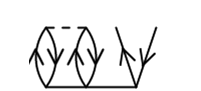
\includegraphics[width=0.25\textwidth]{images/T3toT1.png} & 
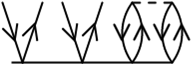
\includegraphics[width=0.25\textwidth]{images/T4toT2.png} \\
$T_3: \braket{ij|ab} t_{ijk}^{abc} \rightarrow T_1$ &
$T_4: \braket{kl|cd} t_{ijkl}^{abcd}  \rightarrow T_2$
\end{tabular}
\end{center}
\caption{Higher order excitations contribute to the energy indirectly by altering $T1$ and $T2$}
\label{fig:higherordercontributions}
\end{figure}
To improve performance, corrections from higher-order t-amplitudes can be calculated via perturbation theory. This mixing of coupled cluster and perturbation theory is used extensively throughout quantum chemistry, and CC singles and doubles with purtubative tipples (CCSD(T)) is currently considered the 'gold-standard' to which other methods can be compared. 

As we are mainly interested in the low-energy part of the spectrum, it can be useful to define an effective hamiltonian, $\bar{H}$, as a similarity transform under $e^T$, 
\begin{align}
\bar{H}&= e^{-T} H e^T\\
\bar{H} \Psi &=E \Psi \label{eq:schroCCeffective}
\end{align}
Such transformations leave eigenvalues unchanged. The coupled cluster equations which must be solved to obtain the t-amplitudes are generated via left-projection of excited states onto  \ref{eq:schroCCeffective}. 
\begin{align}
\begin{split}
\braket{\Phi| \bar{H} |\Phi_0} &= E_{CC}\\
\braket{\Phi^a_i|\bar{H} |\Phi_0} &= 0 \\
\braket{\Phi^{ab}_{ij}|\bar{H} |\Phi_0} &= 0 \\
\vdots
\end{split}
\label{eq:cc_eqatations}
\end{align}
Coupled cluster is size consistent for any level of truncation. That is, for two systems A and B, 
\begin{equation}
E_{AB} = E_{A} + E_{B}
\end{equation}
The main drawback of CC is their prohibitive computational complexity. CCSD, and CCSD(T) formally scale as $\mathcal{O}(n_{occ}^2 n_{vrt}^4)$ and $\mathcal{O}(n_{occ}^3 n_{vrt}^4)$, respectively. Ideally, linear or better scaling is desired. Local-orbital methods work well for finite, non-conjugated, ground state systems while scaling near-linearly. These methods will be described in detail in \cref{sec:EfficientElectronicStructure} There is currently no sub-linear method for excited states, although efficient algorithms do exist. 
\subsubsection{Equation-of-Motion Coupled Cluster}
Originally described in the context of the equivalent time dependent linear-response coupled cluster theory, equation-of-motion coupled cluster (EOM-CC) is best motivated by simultaneously considering two Schr\"odinger equations: one each for a reference wavefunction and an excited state. 
\begin{align}
H \Psi_0 &= E_0 \Psi_0 \label{eq:ground_SE}\\
H \Psi_k &= E_k \Psi_k \label{eq:excited_SE}
\end{align}
The excited state is related to the ground state through the action of some operator, $\hat{R}_k$.
\begin{equation}
\ket{\Psi_{k}} = \hat{R}_k \ket{\Psi_{0}} \label{eq:EOM_excited_state}
\end{equation}
Left multiplying \cref{eq:ground_SE} by $R_k$ and subsequent subtraction from \cref{eq:excited_SE} yields an expression for the energy difference: 
\begin{align}
[H,\hat{R}_k] \ket{\Psi_{0}}  = \Delta E_k \ket{\Psi_{0}} \label{EOM_ansatz}
\end{align}
The simplest way to broach the traditional CC framework is to now chose the reference state to be a CC wavefunction, $\ket{\Psi_{CC}} = e^T \ket{\Phi}$, as in  \cref{eq:CC_wavefunction}, and $\hat{R}$ to be an excitation operator:
\begin{align}
\begin{split}
\hat{R}_k &= \underbrace{\sum r^a_i \{a^\dag i\}}_{R_1} + \underbrace{\sum r^{ab}_{ij} \{a^\dag i b^\dag j\}}_{R_2}+ \dots \\
&=  R_1 + R_2 + \dots \label{eq:R_K}
\end{split}
\end{align}
Using that the excitation operators $\hat{R}$ and $\hat{T}$ commute, \cref{EOM_ansatz} can be re-written in terms of the transformed Hamiltonian and the SCF eigenstate: 
\begin{align}
[H,\hat{R}_k] \ket{\Psi} &= \Delta E_k \, \ket{\Psi} \label{eq:EOM_transformed_basis} \\
[H,\hat{R}_k] e^T \ket{\Phi} &= \Delta E_k \, e^T \ket{\Phi}\notag  \\
[ e^{-T} H e^T, \,\hat{R}_k] \ket{\Phi} &= \Delta E_k \ket{\Phi} \notag\\
[\bar{H}, \hat{R_k}] \ket{\Phi} &= \Delta{E} \hat{R_k} \ket{\Phi} \label{eq:EOM_transformed_hamiltonian} 
\end{align} 

As $\bar{H}$ is non-hermitian, each $R_{k}$ has a left hand eigenvector, $\hat{L}_{k}$, which acts as a deexciation operator. The $\hat{L}_{k}$'s are given by the left eigenvalue problem and intermediate normalization conditions,
\begin{align}
\bra{\Phi} \hat{L}_k \bar{H} = \bra{\Phi}\hat{L}_k \Delta E\\
\braket{\Phi| L_k R_l |\Phi} = \delta_{k,l}\
\end{align}

Unlike $\hat{T}$, the set of $\hat{R}_k$ need not be particle conserving. As a result, different sectors of Fock-space can be made accessible by making different choices for the set of $\hat{R_k}$. Of particular significance are single-electron attachments (EA), ionization potentials (IP), and excitations (EE), which can be selected by choosing $R$ to generate N-1, N+1, and (singly excited) N particle eigenstates: 
\begin{align}
R_{IP} &= \sum r_i \{i\} + \sum r_{ij}^a  \{a^\dag i j\} + ...  \label{eq:RIP}\\ 
R_{EA} &= \sum r^a \{a^\dag \} + \sum r^{ab}_{i} \{a^\dag i b^\dag\} + ... \label{eq:REA}\\
R_{EE} &= \underbrace{\sum r^a_i \{a\dag i\}}_{\text{primary space (P)}} + \underbrace{\sum r^{a,b}_{i,j}  \{a^\dag i b^\dag j\}}_{\text{complementary space(Q)}} + ... \label{eq:REE}
\end{align}

These energies lie within the one hole (IP) one particle (EA) and one particle one hole (EE) sectors of fock space. These equations are decoupled, and can therefore be treated separately. In practice, EE amplitudes are based on preceding IP/EA calculations. To obtain accurate energies, contributions from states with one excitation level above the energies of interest must be included (i.e. 1p2h, 2p1h, 2p2h for IP, EA, and EE, respectively). This so-called complementary (Q) space scales as $N^6$ with the basis and is considerably larger than the primary space (P) defined by the first term in $R_k$. 

\Cref{eq:R_K,eq:RIP,eq:REE,eq:REA} depict EOM-CC as a CI procedure using a transformed CC Hamiltonian: $\hat{R}$ is a CI-like construction of the excitation manifold, and the eigenvalues $\Delta E_k$ are exactly the excitation energies of the excited states $\Psi_k$. The issue of size-extensiveness should then be addressed. The root of the size-extensivity problem in truncated CI are the $\Delta E C_n$ terms. In EOM, the analogous $\Delta E R_n$ terms are explicitly set to zero as a result of the constraints set by the CC equations
\begin{equation}
\textit{I would like to show this algebraicly, need to write it out}
\end{equation}. While not rigorously size-extensive, EOM-CC\textit{will} correctly report extensive properties for states which are within the truncation level of T (e.g. single-electron excitations for EOM-CCSD). The exception is states involving single electron charge-transfer, where an electron on subsystem A is ionized and attached to subsystem B. Such states are described by the 1h+2h1p determinants on A and the 1p+2p1h determinants on B. As a result contributions from overall 3h3p (triply excited) determinants are required. Excited state properties can be defined as energy derivatives and made to scale properly, while ionization potentials and electron attachments are size-intensive, regardless of truncation in $R$ or $T$ 

\begin{equation}
\textit{easy to show diagrammatically but is there a good argument for it outside of diagrammatic analsys?}
\end{equation}.\\

Here will be some EOM-CC results.


\subsubsection{Partitioned EOM-CCSD}
Diagonalization of the transformed Hamiltonian is without doubt the most intensive step. More precisely, diagonalization is dominated by operations involving the $N_{bas}^6$ QQ matrix block (\cref{table:PQspace}). Typically, direct (Davidson) diagonalization is  used, and the slow step involves matrix-vector multiplication of the form $QQ \cdot \hat{v}$. While diagonal QQ elements are too large to be ignored, off-diagonal QQ elements  correspond to e.g. simultaneous double excitations in EE-EOM, and are therefore small. Partitioned EOM-CC exploits this by replacing the QQ block with the diagonal terms of the Fock matrix (\cref{fig:partitioned-EOM}). The complexity reduction due to this approximation is on the order of $\mathcal{O}(Q^3) \rightarrow \mathcal{O}(Q)$. 

\begin{table}[htb]
\centering
\begin{tabular}{c|c|c|c}
\centering
Method & Primary space (P) & Secondary space (Q) & Approximate matrix rank\\
\hline
IP-EOM & 1h & 2h1p  & $N \cdot N^3$\\
EA-EOM & 1p & 2p1h& $N \cdot N^3$\\
EE-EOM & 1p1h & 2p2h &$N^2 \cdot N^4$\\
\end{tabular}
\caption{Primary and secondary spaces of partitioned EOM}
\label{table:PQspace}
\end{table}

\begin{figure}[h]
\[
\left(\begin{array}{@{}c|c@{}}
  PP
  & QP \\
\hline PQ &
\begin{matrix}
\phantom{X}&\phantom{X}&\phantom{X}\\
\phantom{X}&QQ&\phantom{X}\\
\phantom{X}&\phantom{X}&\phantom{X} 
\end{matrix}
\end{array}\right)
\xRightarrow{\hspace{5mm}}
\left(\begin{array}{@{}c|c@{}}
  PP &QP\\
\hline
 PQ &\begin{matrix}
\phantom{X}&\phantom{X}&\phantom{X}\\
\phantom{X}&F \delta_{ij} &\phantom{X}\\
\phantom{X}&\phantom{X}&\phantom{X}
\end{matrix}
\end{array}\right)
\]
\caption{Partitioned EOM-CC reduces computational complexity by replacing the QQ block with the diagonal part of the Fock matrix}
\label{fig:partitioned-EOM}
\end{figure}

Partitioned EOM has proved to give accurate predictions of second-order properties which are dominated by contributions from single excitations. Nooijen et. al. 
\begin{equation}(Chemical Physics Letters 266 (1997) 456-464) 
\end{equation}
have reported NMR chemical 
shifts obtained via partitioned EOM-CC give results comparable to unpartitioned EOM while being much more computationally attractive.\\

I would like more examples of p-EOM-cc in the final draft. Examples are somewhat elusive. I am not sure if partitioned EOM deserves its own section and I may just append it to the previous.  


\subsubsection{STEOM-CCSD}
While EOM-CCSD uses a linear parametrization of the excitation manifold, another approach is to take an exponential parametrization, which results in a doubly-transformed Hamiltonian $G$,
\begin{align}
G =  \hat{\bar{H}} &= \{e^{\hat{S}}\}^{-1} \bar{H} \{e^{\hat{S}}\}\\
 &= \{e^{\hat{S}}\}^{-1} e ^{-T}H e^T \{e^{\hat{S}}\} \\
& = g_0 + \sum_{p,q}g^p_q \{p^\dag q \} + \sum_{p,q,r,s} g_{rs}^{pq}\{p^\dag r q^\dag s\} + \dots
\end{align}
The new operator $\hat{S}$ is defined with respect to a user-chosen active space, and it is required that the STEOM eigenvectors are well represented within this space. Scaling with respect to the active space is modest and as such relatively large active spaces can generally be chosen. In the case that the required active space is prohibitively large, a rotation of the virtuals may help reduce complexity, as the CC equations are invariant with respect to orbital rotations.\\

In the following, $i,j,k,l$ and $a,b,c,d$ denote occupied and virtual orbitals, $p,q,r,s$ denote general orbitals, as usual. Explicitly active particle/hole states will be indicated by a cap ($\cap$) superscript, and explicitly inactive orbitals with cup ($\cup$) superscript, e.g. $i^{\cap}$ is active and $a^{\cup}$ inactive. This notation is reasonably accessible if thought of in terms of light switches. \\
$\hat{S}$ consists of two parts; $\hat{S} = {S}^+ + {S}^-$, which are further broken down into single and double quasi-particle parts.  

\begin{align}
\hat{S}^+ &= \hat{S}^+_1 + \hat{S}^+_2 =  \sum_{a^{\cup}, b^{\cap}} S^{a^{\cup}}_{b^{\cap}} \{a^{\cup\dag} b^{\cap} \} + \frac{1}{2} \sum_{a,b,c^{\cap},i} S^{a,b}_{i,c^{\cap}} \{a^\dag i b^{\dag} c^{\cap}\} \\
\hat{S}^- &= \hat{S}^-_1 + \hat{S}^-_2 = \sum_{i^{\cup}, j^{\cap}}  S\,^{j^{\cap\dag}}_{i^{\cup}} \{j^{\cap\dag} i^{\cup} \}  + \frac{1}{2}\sum_{i, j, a, k^{\cap}} S^{ak^\cap}_{ij} \{ a^{\dag} i k^{\cap\dag} j \} 
\end{align}  

The s-amplitudes are built using operators which create electrons in occupied orbitals ($i^\dag$) and destroy electrons in unoccupied orbitals($a$). Under second quantization, the action of $i^\dag$ and $a$ destroy the particle-hole quasi-particles produced by excitation operators. As the reference state, by definition, contains no quasi-particles, reference state will always vanish under action of S. Thus non-zero $S$ amplitudes must describe the coupling between excited determinants. This can be readily shown by examining how the construction of $S$ constraints elements of $\hat{G}$. 
\begin{align}
g_i^a &= g_i^{ab} = 0 \label{eq:STEOM-CCSD}\\
S^+ \rightarrow g^{b^{\cup}}_{a^{\cap}}& = g^{ab}_{ic^{\cap}} =0 \label{eq:STEOM-splus}\\
S^- \rightarrow g^{i^{\cap}}_{i^{\cup}} &= g^{ai^{\cap}}_{jk} =0 \label{eq:STEOM-sminus} 
\end{align}
\Cref{eq:STEOM-CCSD} is equivalent to the CCSD equations, while the constraints set in \cref{eq:STEOM-splus} and \cref{eq:STEOM-sminus} define the $S^+$ and $S^-$ operators, respectively. Projecting G against states which would typically survive the action of, for example, $g^{ai^{\cap}}_{jk}$, allows for physical interpretation of these constraints:
\begin{align}
g^{ai^{\cap}}_{jk} \equiv \braket{\Phi^a_{jk}|G|\Phi_{i^{\cap}}} = 0
\end{align}
$g^{ai^{\cap}}_{jk}$ describes coupling between active 1h states and 2h1p states. This interaction is required to vanish, and thus the amplitude equations explicitly decouple excitation blocks from higher excitations. The $G$ amplitudes are typically obtained by solving the IP/EA-EOMCC equations, followed by a normalization procedure described by an eigenvalue problem in $S$ \\

By definition, $G$ is approximately upper triangular with respect to excitation blocks. Defining the primary space as the reference determinant plus single excitations, 
\begin{equation}
G = 
\begin{blockarray}{ccccc}
 &\ket{0} & \ket{S} & \ket{D} & \ket{T}  \\
\begin{block}{c(cccc)}
\bra{0} & E_{CC} & X & X & 0 \\
\bra{S} &0 & X & X & X \\
\bra{D} & 0 & \sim & X & X \\
\bra{T} & \sim & \sim& \sim& X \\
\end{block}
\end{blockarray}
\rightarrow \begin{pmatrix}
\mathbf{PP} & \mathbf{PQ} \\
\mathbf{\approx 0} & \mathbf{QQ} \\
\end{pmatrix}
\end{equation}
\\ Where $\sim$ indicates small matrix elements, and X indicates elements of typical magnitude. Solving the $G$ amplitude equations is equivalent to diagonalizing G over the excitation manifold, as is the case in EOM-CC. 

The main draw of STEOM is two-fold: because the QP block is transformed to zero, each excitation block can be diagonalized separately. Excitation energies can be extracted directly from $PP$, while traditional EE-EOM requires diagonalization of the QQ space. Furthermore, EE-STEOM-CCSD is comparable to EE-EOM-CCSD(T) in accuracy because expansion of the exponential and projection over the primary space yeilds an implicit tripples correction 
\begin{equation}
\{S^+_2 S^-_2\}\ket{\phi_a^i} + S_2 \ket{\Phi^{ab}_{ij}} \label{eq:implicit_trip}
\end{equation}
The resulting terms must be triply excited states, as the operation of $S_2$ increases net excitation by one level. Diagrams of the second term are given below to further show this result:
\begin{equation*}
S_2 \ket{\Phi^{ab}_{ij}} =  \begin{gathered}
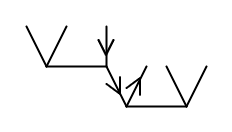
\includegraphics[width=0.25\textwidth]{images/SM.png} 
\end{gathered}
+
\begin{gathered}
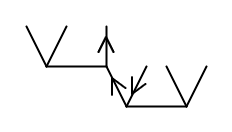
\includegraphics[width=0.25\textwidth]{images/SP.png} 
\end{gathered}
\end{equation*}
The connectedness of \cref{eq:implicit_trip} guarantees size-extensive results for charge-transfer states without explicit treatment of the QQ space. 
